%%%%%%%%%%%%%%%%%%%%%%%%%%%%%%%%%%%%%%%%%
% WU Poster
% LaTeX Template
% Version 1.0 (08/12/2019)
% (Based on Version 1.0 (08/12/2019) of the  Nicolas Ballarini Poster
%
% License:
% CC BY-NC-SA 4.0 (https://creativecommons.org/licenses/by-nc-sa/4.0/)
%
% Created by:
% Clemens Leitner, Student@TU Wien
% clemens.georg.leitner@gmail.com
% https://velocit.at/
%%%%%%%%%%%%%%%%%%%%%%%%%%%%%%%%%%%%%%%%%


\def\footer#1{\def\insertfooter{#1}}
%--------------------------------------------------------------------------------------
%	PACKAGES AND OTHER DOCUMENT CONFIGURATIONS
%--------------------------------------------------------------------------------------

\documentclass[final, border=3pt]{beamer}



\usepackage[scale=1.150]{beamerposter} % Use the beamerposter package
\usetheme{WUposter} % Use the WUposter theme supplied with this template

% Include a logo of your project if desired
\logo{\pgfputat{\pgfxy(-11,107)}{\pgfbox[center,base]{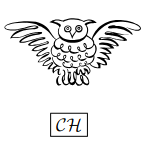
\includegraphics[width=7cm]{ProjectLogo.png}}}}  

\usepackage{multicol}
\usepackage{array}
%The following two are column definitions for the aknowledgements section
\newcolumntype{L}{>{\arraybackslash}m{22cm}}
\newcolumntype{S}{>{\arraybackslash}m{5cm}}
\usepackage{pgf}  
\usepackage{mathtools}
\usepackage{amsmath, amsthm, amssymb, amsfonts}
\usepackage{braket}
\usepackage{exscale}
\usepackage{xcolor}
\usepackage{ushort}
\usepackage{setspace}
\usepackage[square,numbers]{natbib}
\usepackage{url}
\bibliographystyle{abbrvnat}
\renewcommand{\vec}[1]{\ushort{#1}}
\renewcommand{\vec}[1]{\mathbf{#1}}
\definecolor{hellblauWU}{RGB}{183,0,229} 
\definecolor{dunkelblauWU}{RGB}{117,0,146} 

%-----------------------------------------------
%  START Set the colors
%  Uncomment to apply colors you want to use.
%-----------------------------------------------
\colorlet{themecolor}{dunkelblauWU}
\usebackgroundtemplate{
\includegraphics{WU_dunkelblau.pdf}}

%\colorlet{themecolor}{hellblauWU}
%\usebackgroundtemplate{\includegraphics{WU_hellblau.pdf}}

%-----------------------------------------------
%  END Set the colors
%-----------------------------------------------


%-----------------------------------------------
%  START Set the width of the columns
%-----------------------------------------------
\setlength{\paperwidth}{84.6cm} % A0 width: 119.4cm with 3mm blead on each side
\setlength{\paperheight}{119.4cm} % A0 height: 84.6cm with 3mm blead on each side
\newlength{\sepmargin}
\newlength{\sepwid}
\newlength{\onecolwid}
\newlength{\twocolwid}
\newlength{\threecolwid}

% The following measures are used for 2 columns
\setlength{\sepmargin}{0.055\paperwidth} % Separation width (white space) between columns
\setlength{\sepwid}{0.03\paperwidth} % Separation width (white space) between columns
\setlength{\onecolwid}{0.43\paperwidth} % Width of one column
\setlength{\twocolwid}{0.9\paperwidth} % Width of two columns

%-----------------------------------------------------------
% The following measures are used for 3 columns
%\setlength{\sepmargin}{0.06\paperwidth} % Separation width (white space) between columns
%\setlength{\sepwid}{0.02\paperwidth} % Separation width (white space) between columns
%\setlength{\onecolwid}{0.28\paperwidth} % Width of one column
%\setlength{\twocolwid}{0.58\paperwidth} % Width of two columns
%\setlength{\threecolwid}{0.88\paperwidth} % Width of three columns
%\setlength{\columnsep}{30pt}

%-----------------------------------------------
%  END Set the width of the columns
%-----------------------------------------------

\usepackage{tikz}
\usepackage{siunitx}
\usepackage{amsmath} % for \text
\usepackage{mathrsfs} % for \mathscr
\usepackage{xfp} % higher precision (16 digits?)
\usepackage[outline]{contour} % glow around text
\usetikzlibrary{decorations.markings,decorations.pathmorphing}
\usetikzlibrary{angles,quotes} % for pic (angle labels)
\usetikzlibrary{arrows.meta} % for arrow size
\contourlength{1.4pt}

\newcommand{\calI}{\mathscr{I}} %\mathcal
\tikzset{>=latex} % for LaTeX arrow head
\colorlet{myred}{red!80!black}
\colorlet{myblue}{blue!80!black}
\colorlet{mygreen}{green!80!black}
\colorlet{mydarkred}{red!50!black}
\colorlet{mydarkblue}{blue!50!black}
\colorlet{mylightblue}{mydarkblue!6}
\colorlet{mypurple}{blue!40!red!80!black}
\colorlet{mydarkpurple}{blue!40!red!50!black}
\colorlet{mylightpurple}{mydarkpurple!80!red!6}
\colorlet{myorange}{orange!40!yellow!95!black}
\tikzstyle{cone}=[mydarkblue,line width=0.2,top color=blue!60!black!30,
                  bottom color=blue!60!black!50!red!30,shading angle=60,fill opacity=0.9]
\tikzstyle{cone back}=[mydarkblue,line width=0.1,dash pattern=on 1pt off 1pt]
\tikzstyle{world line}=[myblue!60,line width=0.4]
\tikzstyle{world line t}=[mypurple!60,line width=0.4]
\tikzstyle{particle}=[mygreen,line width=0.5]
\tikzstyle{photon}=[-{Latex[length=4,width=3]},myorange,line width=0.4,decorate,
                    decoration={snake,amplitude=0.9,segment length=4,post length=3.8}]
\tikzstyle{singularity}=[myred,line width=0.6,decorate,
                         decoration={zigzag,amplitude=2,segment length=6.17}]
\tikzset{declare function={%
  penrose(\x,\c)  = {\fpeval{2/pi*atan( (sqrt((1+tan(\x)^2)^2+4*\c*\c*tan(\x)^2)-1-tan(\x)^2) /(2*\c*tan(\x)^2) )}};%
  penroseu(\x,\t) = {\fpeval{atan(\x+\t)/pi+atan(\x-\t)/pi}};%
  penrosev(\x,\t) = {\fpeval{atan(\x+\t)/pi-atan(\x-\t)/pi}};%
  kruskal(\x,\c)  = {\fpeval{asin( \c*sin(2*\x) )*2/pi}};% Penrose coordinates for Kruskal
}}
\def\tick#1#2{\draw[thick] (#1) ++ (#2:0.04) --++ (#2-180:0.08)}
\def\Nsamples{20} % number samples in plot

% LIGHTCONE
\def\R{0.08} % size lightcone
\def\e{0.08} % vertical scale
\def\ang{45} % angle light cone
\def\angb{acos(sqrt(\e)*sin(\ang))} % angle ellipse center to point of tangency
\def\a{\R*sin(\ang)*sqrt(1-\e*sin(\ang)^2)/(1-\e*sin(\ang)^2)} % vertical radius
\def\b{\R*sqrt(\e)*sin(\ang)*cos(\ang)/(1-\e*sin(\ang)^2)} % horizontal radius
\def\coneback#1{ % light cone part to be drawn behind world lines
  \draw[cone back] % dashed line back
    (#1)++(-45:\R) arc({90-\angb}:{90+\angb}:{\a} and {\b});
  \draw[cone,shading angle=-60] % top edge & inside
    (#1)++(0,{\R*cos(\ang)/(1-\e*sin(\ang)^2)}) ellipse({\a} and {\b});
}
\def\conefront#1{ % light cone part to be drawn over world lines
  \draw[cone] % light cone outside
    (#1) --++ (45:\R) arc({\angb-90}:{-90-\angb}:{\a} and {\b})
     --++ (-45:2*\R) arc({90-\angb}:{-270+\angb}:{\a} and {\b}) -- cycle;
}


%--------------------------------------------------------------------------------------
%	TITLE SECTION 
%--------------------------------------------------------------------------------------
\setbeamertemplate{title}[left]
\setbeamertemplate{frametitle}[default][left]
%\setmainfont{Georgia}

\title{The Unruh effect and it's generalization to curved spacetimes} % Poster title

\author{Carlos H. Correr, André G. S. Landulfo} % Author(s)

\institute{Institute of Physics, University of São Paulo} % Institution(s)
%--------------------------------------------------------------------------------------

\begin{document}

  \addtobeamertemplate{block end}{}{\vspace*{1ex}} % White space under blocks
  \addtobeamertemplate{block alerted end}{}{\vspace*{0ex}} % White space under highlighted (alert) blocks
  \setlength{\belowcaptionskip}{2ex} % White space under figures
  \setlength\belowdisplayshortskip{1ex} % White space under equations
  
  
    \begin{frame}[t] % The whole poster is enclosed in one beamer frame

        \begin{columns}[t] % The whole poster consists of two major columns
	  
            \begin{column}{\sepmargin}\end{column}
      
	        \begin{column}{\onecolwid} % The first column
          
                \begin{block}{Unruh effect in Minkowski}
                    In the formulation of quantum field theory in curved spacetimes, the particle concept is observer-dependent. For stationary spacetimes, it can be built with the aid of timelike Killing vector fields. The high degree of symmetry in Minkowski spacetime time, described by the metric
                    \begin{equation}
                        \mathrm{d}s^2=-\mathrm{d}t^2+\mathrm{d}x^2+\mathrm{d}y^2+\mathrm{d}z^2,
                    \end{equation}
                    allows many possible Killing fields, consider the following two
                    \begin{equation}
                        \xi^a=\left(\partial_t\right)^a\hspace{2cm}\text{and}\hspace{2cm}\chi^a=a\left[x\left(\partial_t\right)^a+t\left(\partial_x\right)^a\right].
                    \end{equation}
                    Observers that follows the orbits of \(\chi^a\) can be interpreted as being uniformly accelerated. The second Killing field separates the spacetime in four regions, with the boundaries being the surfaces where it is null, \(\mathfrak{h}_A\) and \(\mathfrak{h}_B\):
                    \begin{equation}
                        \begin{aligned}
                            &\text{Region I}=I^-\left(\mathfrak{h}_A\right)\cap I^+\left(\mathfrak{h}_B\right)\hspace{2cm}\text{Region II}=I^+\left(\mathfrak{h}_A\right)\cap I^-\left(\mathfrak{h}_B\right)\\
                            &\text{Region III}=J^-(S)\hspace{6.9cm}\text{Region IV}=J^+(S)
                        \end{aligned}.
                    \end{equation}

                    \begin{figure}[h]
                        \begin{tikzpicture}[scale=8]
                            \message{Penrose diagram (45 rotation)^^J}
                            
                            \def\R{0.10} % size lightcone
                            \def\Nlines{6} % number of world lines (at constant r/t)
                            \pgfmathsetmacro\d{0.92/\Nlines} % grid size
                            
                            \coordinate (O) at (0,0);
                            \coordinate (W) at (-1.05,0);
                            \coordinate (E) at (1.15,0);
                            \coordinate (S) at (0,-1.05);
                            \coordinate (N) at (0,1.15);
                            \coordinate (SW) at (-135:1.45);
                            \coordinate (SE) at (-45:1.45);
                            \coordinate (NW) at (135:1.45);
                            \coordinate (NE) at (45:1.45);
                            \coordinate (X0) at (-0.41,-1);
                            \coordinate (X1) at (-\d,-3*\d);
                            \coordinate (X2) at (2*\d,2*\d);
                            \coordinate (X3) at (0.54,1);
                            
                            % WORLD LINES GRID
                            \message{Making world lines...^^J}
                            \foreach \i [evaluate={\x=\i*\d;}] in {1,...,\Nlines}{
                                \message{  Running i/N=\i/\Nlines, x=\x...^^J}
                                \draw[world line]   (-\x,-1) -- (-\x,1);
                                \draw[world line]   ( \x,-1) -- ( \x,1);
                                \draw[world line t] (-1,-\x) -- (1,-\x);
                                \draw[world line t] (-1, \x) -- (1, \x);
                            }
                            
                            % AXES
                            \draw[->,thick,mydarkblue!70!black]
                                (W) -- (E) node[left=4,below=0] {$S$};
                            \draw[->,thick,mydarkpurple!70!black]
                                (S) -- (N) coordinate (N) node[below=4,left=0] {$t$};
                            \draw[->,thick,mydarkred] (SW) -- (NE) node[below right=-2] {$V=x+t$};
                            \draw[->,thick,mydarkred] (SE) -- (NW) node[below left=-2] {$U=t-x$};
                            
                            % INFINITY LABELS
                            \node[above=1,left=1,mydarkblue] at (W) {$i^0$};
                            \node[above=1,right=1,mydarkblue] at (E) {$i^0$};
                            \node[right=3,below=2,mydarkpurple] at (0,-1) {$i^-$};
                            \node[right=3,above=0,mydarkpurple] at (N) {$i^+$};
                            \node[mydarkblue,left=5,below right=-1] at (SE) {$\calI^-$};
                            \node at (126:0.89) {\(\mathfrak{h}_B\)};
                            \node at (39:0.9) {\(\mathfrak{h}_A\)};
                            \node[mydarkblue,right=8,below left=-1] at (SW) {$\calI^-$};
                            \node[mydarkblue,left=5,above right=-1] at (NE) {$\calI^+$};
                            \node[mydarkblue,right=8,above left=-1] at (NW) {$\calI^+$};
                            
                            % LIGHT CONE BACK
                            \coneback{X1};
                            \coneback{X2};
                            
                            % PARTICLE
                            \draw[particle,decoration={markings,mark=at position 0.170 with {\arrow{latex}},
                                                                mark=at position 0.505 with {\arrow{latex}},
                                                                mark=at position 0.860 with {\arrow{latex}}},postaction={decorate}]
                                (X0) to[out=70,in=-110] (X1) to[out=70,in=-110] (X2) to[out=70,in=-120] (X3);
                            
                            % LIGHT CONE FRONT
                            \conefront{X1};
                            \conefront{X2};
                            
                        \end{tikzpicture}
                    \end{figure}
                    On \(\mathfrak{h}_A\) (\(\mathfrak{h}_B\)), modes are positive-frequency with respect to retarded (advanced) time \(V\;(U)\) if, and only if, they are positive-frequency with respect to the inertial one \(t\). Moreover, the Killing time \(v\) (\(u\)) induced by \(\chi^a\) are related to the inertial ones on \(\mathfrak{h}_A\) (\(\mathfrak{h}_B\)) by
                    \begin{equation}
                        v=\frac{1}{a}\ln{\lvert V\rvert}\hspace{2cm}\text{and}\hspace{2cm}u=-\frac{1}{a}\ln{\lvert U\rvert}.
                    \end{equation}
                    Analyzing pure positive frequencies on the horizon, allows us to find a Bogoliubov transformation \(S\) that relate the two possible constructions. If \(\ket{0}_M\) represents the Minkowski inertial vacuum, we have
                    \begin{equation}
                        S\ket{0}_M=\prod_{j}\left(\sum_{n=0}^{\infty}e^{-\frac{\pi n\omega_j}{a}}\ket{n_j}_I\otimes\ket{n_j}_{II}\right),
                    \end{equation}
                    where \(\ket{n_j}_I\) represents a state with \(n\) particles in the basis mode \(\{\psi^{I}_{j}\}\) of region I, the same stands for region II. The density matrix restricted to region I is
                    \begin{equation}
                        \rho^I=\prod_j\left(\sum_{n=0}^{\infty}e^{-\frac{2n\omega_j}{a}}\ket{n_j}_I\bra{n_j}_I\right).
                    \end{equation}
                    This result is compatible with the statement that uniformly accelerated observers interpret the Minskowski vacuum as a thermal bath of particles at a temperature

                    \begin{equation}
                        T=\frac{a}{2\pi}\cong \frac{a}{10^{19}\unit{\meter\per\second^2}}\unit{\kelvin}.
                    \end{equation}
                \end{block}

            \end{column}
                  
                  
                  
            \begin{column}{\sepwid}  \end{column}

         
        \begin{column}{\onecolwid} %The second column
          
            \begin{block}{Unruh effect in curved spacetimes}
                The main feature used to derive the Unruh effect is the existence of the surfaces \(\mathfrak{h}_A\) and \(\mathfrak{h}_B\). Such a structure can be generalized by bifurcate Killing horizon, associated with a Killing field \(\xi^a\), that induce a spacetime separation as in the previous description. 
                In this case, the surface gravity of the horizon, \(\kappa\), plays a key role. It is given by
                \begin{equation}
                    \kappa=\lim_{\mathfrak{h}}(a\xi),
                \end{equation}
                where \(a\) is the norm of the 4-acceleration of a observer whose worldline is one orbit of \(\xi^a\). Moreover, we can use it, together with the induced Killing time \(v\;(u)\), to obtain an affine parameter \(V\;(U)\) for the null geodesics that generate the horizons. The expressions obtained are
                \begin{equation}
                    v=\frac{1}{\kappa}\ln{\lvert V\rvert}\hspace{2cm}\text{and}\hspace{2cm}u=-\frac{1}{\kappa}\ln{\lvert U\rvert}.
                \end{equation}
                Henceforth, we pick a pure, quasifree state that is non-singular and invariant under the isometries generated by \(\xi^a\) to be the vacuum state. Then, due to the same procedure done in Minkowski, we find that observers that follows the orbits of the Killing field perceive this vacuum state as a particles thermal bath at a temperature
                \begin{equation}
                    T=\frac{\kappa}{2\pi}.
                \end{equation}

                For example, consider the extended Schwarschild spacetime whose metric is
                \begin{equation}
                    \mathrm{d}s^2=-\left(1-\frac{2M}{r}\right)\mathrm{d}t^2+\left(1-\frac{2M}{r}\right)^{-1}\mathrm{d}r^2+r^2\mathrm{d}\Omega^2.
                \end{equation}

                \begin{figure}
                    \begin{tikzpicture}[scale=8]
                        \message{Extended Penrose diagram: Schwarzschild black hole^^J}
                        
                        \def\R{0.08} % size lightcone
                        \def\Nlines{3} % number of world lines (at constant r/t)
                        \pgfmathsetmacro\ta{1/sin(90*1/(\Nlines+1))} % constant r/t value 1
                        \pgfmathsetmacro\tb{sin(90*2/(\Nlines+1))}   % constant r/t value 2
                        \pgfmathsetmacro\tc{1/sin(90*2/(\Nlines+1))} % constant r/t value 3
                        \pgfmathsetmacro\td{sin(90*1/(\Nlines+1))}   % constant r/t value 4
                        \coordinate (-O) at (-1, 0); % center III: origin (r,t) = (0,0)
                        \coordinate (-S) at (-1,-1); % south III: t=-infty, i-
                        \coordinate (-N) at (-1, 1); % north III: t=+infty, i+
                        \coordinate (-W) at (-2, 0); % east III:  r=-infty, i0
                        \coordinate (-E) at ( 0, 0); % west III:  r=+infty, i0
                        \coordinate (O)  at ( 1, 0); % center I: origin (r,t) = (0,0)
                        \coordinate (S)  at ( 1,-1); % south I: t=-infty, i-
                        \coordinate (N)  at ( 1, 1); % north I: t=+infty, i+
                        \coordinate (E)  at ( 2, 0); % east I:  r=-infty, i0
                        \coordinate (W)  at ( 0, 0); % west I:  r=+infty, i0
                        \coordinate (B)  at ( 0,-1); % singularity bottom
                        \coordinate (T)  at ( 0, 1); % singularity top
                        \coordinate (X0) at ({asin(sqrt((\ta^2-1)/(\ta^2-\tb^2)))/90},
                                            {-acos(\ta*sqrt((1-\tb^2)/(\ta^2-\tb^2)))/90}); % particle 1
                        \coordinate (X1) at ({asin(sqrt((\tc^2-1)/(\tc^2-\td^2)))/90},
                                            {acos(\tc*sqrt((1-\td^2)/(\tc^2-\td^2)))/90}); % particle 2
                        \coordinate (X2) at (45:0.87); % particle falling in BH horizon
                        \coordinate (X3) at (0.60,1.05); % particle falling in BH singularity
                        
                        \begin{scope}
                            
                            % CLIP to fill inside zigzag lines
                            \clip[decorate,decoration={zigzag,amplitude=2,segment length=6.17}]
                            (S) -- (-S) --++ (-1.1,-0.1) |-++ (4.2,2.2) |- cycle;
                            \clip[decorate,decoration={zigzag,amplitude=2,segment length=6.17}]
                            (-N) -- (N) --++ (1.1,0.1) |-++ (-4.2,-2.2) |- cycle;
                            
                            % REGIONS FILLS
                            \fill[mylightpurple] (-N) |-++ (2,0.1) -- (N) -- (-S) -- (S) -- cycle;
                            \fill[mylightpurple] (-S) |-++ (2,-0.1) -- (S) -- (-N) -- (N) -- cycle;
                            
                            \fill[mylightblue] (-N) -- (-E) -- (-S) -- (-W) -- cycle;
                            \fill[mylightblue] (N) -- (E) -- (S) -- (W) -- cycle;
                            
                            % CONE BACK
                            \coneback{X0};
                            \coneback{X1};
                            \coneback{X2};
                            
                            % WORLD LINES
                            \draw[world line] (-N) -- (-S) (N) -- (S);
                            \draw[world line t] (-W) -- (-E) (W) -- (E) (0,-1.1) -- (0,1.1);
                            \message{Making world lines...^^J}
                            \foreach \i [evaluate={\c=\i/(\Nlines+1); \cs=sin(90*\c);}] in {1,...,\Nlines}{
                            \message{  Running i/N=\i/\Nlines, c=\c, cs=\cs...^^J}
                            \draw[world line t,samples=2*\Nsamples,smooth,variable=\x,domain=-2:2] % region I/III, constant t
                                plot(\x,{-kruskal(\x*pi/4,\cs)})
                                plot(\x,{ kruskal(\x*pi/4,\cs)});
                            \draw[world line,samples=\Nsamples,smooth,variable=\y,domain=0:2] % region I/III, constant r
                                plot({-1-kruskal(\y*pi/4,\cs)},\y-1)
                                plot({-1+kruskal(\y*pi/4,\cs)},\y-1)
                                plot({1-kruskal(\y*pi/4,\cs)},\y-1)
                                plot({1+kruskal(\y*pi/4,\cs)},\y-1);
                            \draw[world line,samples=\Nsamples,smooth,variable=\x,domain=0:2] % region II/IV, constant r
                                plot(\x-1,{kruskal(\x*pi/4,\cs)-1})
                                plot(\x-1,{1-kruskal(\x*pi/4,\cs)});
                            \draw[world line t,samples=\Nsamples,smooth,variable=\y,domain=-1.05:1.05] % region II/IV constant t
                                plot({-kruskal(\y*pi/4,\cs)},\y)
                                plot({ kruskal(\y*pi/4,\cs)},\y);
                            }
                            
                            % PARTICLE WORLD LINE
                            \draw[particle,decoration={markings,mark=at position 0.16 with {\arrow{latex}},
                                                                mark=at position 0.45 with {\arrow{latex}},
                                                                mark=at position 0.72 with {\arrow{latex}},
                                                                mark=at position 0.90 with {\arrow{latex}}},postaction={decorate}]
                            (S) to[out=77,in=-70] (X0) to[out=110,in=-80] (X1)
                                to[out=100,in=-90] (X2) to[out=75,in=-80] (X3);
                            
                        \end{scope}
                        
                        % REGIONS
                        \node[fill=mylightblue,inner sep=2] at (-O) {III};
                        \node[fill=mylightblue,inner sep=2] at (O) {I};
                        \node[fill=mylightpurple,inner sep=2] at (0,0.64) {II};
                        \node[fill=mylightpurple,inner sep=2] at (0,-0.64) {IV};
                        
                        % INFINITY LABELS
                        \node[above=1,left=1,mydarkblue] at (-2,0) {$i^0$};
                        \node[above=1,right=1,mydarkblue] at (2,0) {$i^0$};
                        \node[right=1,below=1,mydarkpurple] at (-S) {$i^-$};
                        \node[right=1,above=1,mydarkpurple] at (-N) {$i^+$};
                        \node[right=1,below=1,mydarkpurple] at (S) {$i^-$};
                        \node[right=1,above=1,mydarkpurple] at (N) {$i^+$};
                        \node[mydarkblue,below left=-1] at (-1.5,-0.5) {$\calI^-$};
                        \node[mydarkblue,above left=-1] at (-1.5,0.5) {$\calI^+$};
                        \node[mydarkblue,above right=-1] at (1.5,0.5) {$\calI^+$};
                        \node[mydarkblue,below right=-1] at (1.5,-0.5) {$\calI^-$};
                        
                        % LIGHT CONE FRONT
                        \conefront{X0};
                        \conefront{X1};
                        \conefront{X2};
                        
                        % ESCAPING PHOTONS
                        \draw[photon] (X0) ++ (45:0.1) --++ (45:0.3);
                        \draw[photon] (X1) ++ (45:0.1) --++ (45:0.3);

                        % BOUNDARIES
                        \draw[singularity] (-N) -- node[above] {$r=0$} (N);
                        \draw[singularity] (S) -- node[below] {$r=0$} (-S);
                        \path (S) -- (W) node[mydarkblue,pos=0.50,below=-2.5,rotate=-45,scale=0.85]
                            {\contour{mylightpurple}{$r=2M$}};
                        \path (W) -- (N) node[mydarkblue,pos=0.32,above=-2.5,rotate=45,scale=0.85]
                            {\contour{mylightpurple}{$r=2M$}};
                        \draw[thick,mydarkblue] (-N) -- (-E) -- (-S) -- (-W) -- cycle;
                        \draw[thick,mydarkblue] (N) -- (E) -- (S) -- (W) -- cycle;

                    \end{tikzpicture}
                \end{figure}
                We pick the Killing field \(\xi^a=\left(\partial_t\right)^a\) that leads to an acceleration \(a^{\mu}=M/r^2\left(\partial_r\right)^{\mu}\). Therefore, we find
                \begin{equation}
                    a\xi=\frac{M}{r^2},
                \end{equation}
                then, the surface gravity of the event horizon is
                \begin{equation}
                    \kappa=\lim_{r\to2M}\frac{M}{r^2}=\frac{1}{4M}.
                \end{equation}
                Thus, if the field state is in the Hartle-Hawking vacuum (a state that satisfies all the required conditions), observers in the orbits of \(\xi^a\) ought to see a particle thermal bath at temperature
                \begin{equation}
                    T=\frac{1}{8\pi M}\cong\frac{6\times10^{-8}M_{\odot}}{M}\unit{K}.
                \end{equation}
		    \end{block}
        \end{column}
      
        \begin{column}{\sepmargin} \end{column}
        \end{columns} 
       
      \begin{columns}[t] % Split up the two columns wide column again
      
      \begin{column}{\sepmargin} \end{column}
            \begin{column}{\onecolwid} % The first column
                \begin{block}{\large Contact information}
                    \vspace*{-0.5cm}
					\begin{footnotesize}
					\begin{itemize}
						\item \href{mailto:carloscorrer@usp.br}{carloscorrer@usp.br}
					\end{itemize}
					\end{footnotesize}	
                \end{block}
		    \end{column} % End of the first column
			\begin{column}{\sepwid}\end{column} % Empty spacer column
			\begin{column}{\onecolwid} % Begin a column 
                \begin{block}{\large References}
			        \vspace*{-0.5cm}
              	    \nocite{*} % Insert publications even if they are not cited in the poster
					{\footnotesize
                    	%\bibliographystyle{plainurl}
						\bibliography{bibliog.bib}}
				\end{block}
			\end{column} % End of the second column
			\begin{column}{\sepmargin}\end{column} % Empty spacer column
            
\end{columns} % End of all the columns in the poster

\begin{columns}
    \begin{column}{8cm}
        \vspace*{-0.9cm}
        \begin{figure}
            
\includegraphics[width=1.1\linewidth]{logo-ifusp.png}
        \end{figure}
    \end{column}
    \begin{column}{8cm}
        \vspace*{-0.9cm}
        \begin{figure}
            
\includegraphics[width=1.1\linewidth]{logo-fapesp.png}
        \end{figure}
    \end{column}
    \begin{column}{6cm}
        \vspace*{-0.7cm}
        \begin{figure}
            
\includegraphics[width=0.8\linewidth]{logo-ufabc.png}
        \end{figure}
    \end{column}
\end{columns}


\end{frame} % End of the enclosing frame

\end{document}
